\documentclass[a4paper,12pt]{article}
\usepackage{tabularx}
\usepackage{hyperref}
\usepackage{multirow}
\usepackage{graphicx}
\usepackage{caption} 
\usepackage{amsmath}


\title{Heating task Report}
\author{Macarena Burguera Perello(\textit{s243296}), \\
        Levente Buzga (\textit{s242964}), \\
        Attila István Kiri (\textit{s242965})}


\begin{document}

\maketitle


\section{Introduction}

In this report, we present the development and optimization of a Python-based simulation designed to evaluate the effectiveness of the Wall Heating concept, as part of the 02613 Python and High-Performance Computing course mini-project. Our primary objective is to create a solution that is both scalable and computationally efficient, enabling rapid evaluation across a large dataset. While we address all the questions outlined in the project description, some tasks are combined where it improves clarity and cohesion.

\section{Tasks}

In this project, we focus on developing and optimizing a Python-based simulation to evaluate the effectiveness of a novel heating method called Wall Heating, which uses interior walls as heat sources. Using the Modified Swiss Dwellings dataset, we simulate heating performance across thousands of building floorplans while prioritizing efficient code execution. The main goal is to ensure that our implementation is both scalable and computationally efficient to enable rapid evaluation across a large dataset.

\subsection{Task 1}

The data provided in the Modified Swiss Dwellings dataset is in a npy format, which is a numpy array format. To load the data we created a python script that uses the numpy library.
Each building has an ID which is stored in \texttt{building\_ids.txt}, 
and two corresponding to the floor plan:

Interior: This file contains a NumPy array with a binary mask. It is 1 for all
interior grid points (i.e., grid points inside a room) and 0 for all other grid points (i.e., grid points
on walls and outside the building
And one for the heating 

Domain: This file contains a NumPy array with the initial conditions for the
simulation grid u. Grid points on load bearing walls have been been set to 5 and grid points on
inside walls to 25. All other points have been set to 0.
This is shown in Figure~\ref{fig:combined_plot}.

\begin{figure}[h!]
        \centering
        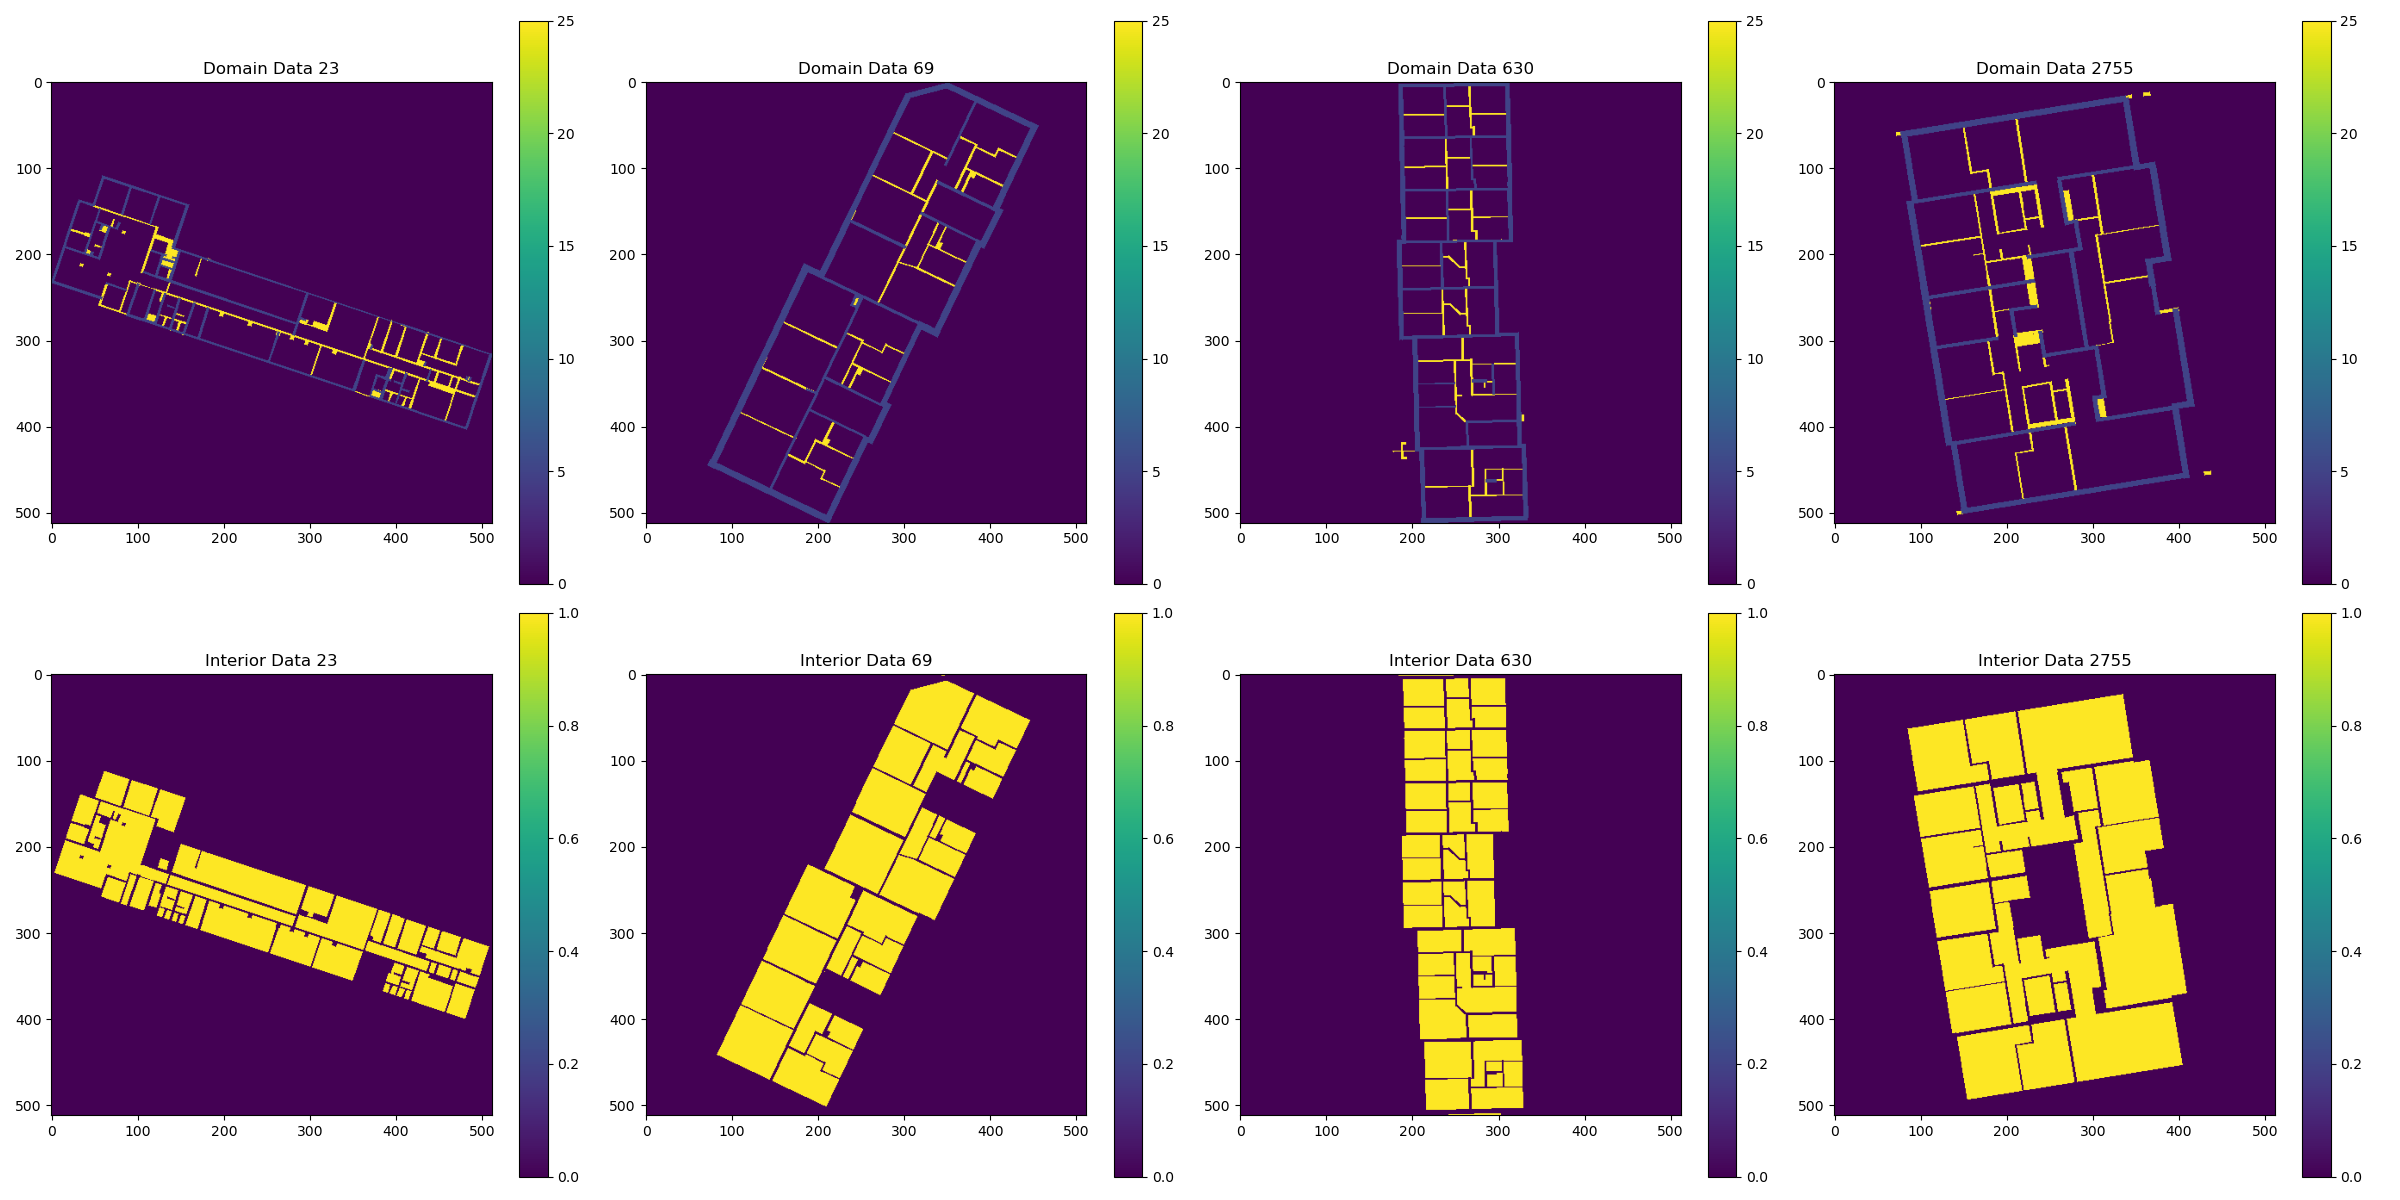
\includegraphics[width=1\textwidth]{Plots/combined_plot.png}
        \caption{Visualization of the dataset: Building IDs, floor plans, and heating domains.}
        \label{fig:combined_plot}
\end{figure}

\subsection{Task 2}
When trying to run the simulation on 20 input files, we timed around 215 seconds. We know there is 4571 different building IDs which means the program should be ran for that amount of times which if we take our previous time it would be estimately:
\[
\text{Total time for 4571 buildings: } T_{\text{total}} = \frac{4571}{20} \times 215
\]

\[
T_{\text{total}} = 49191.25 \text{ seconds} = 819.85 \text{ minutes} = 13.66 \text{ hours}
\]
This shows that the simulation is not efficient enough to run on a large dataset. We need to optimize the code to reduce the time taken for each simulation.


\subsection{Task 3}
Now that we ran the simulation we can start analyzing the results. In the output we can find 4 different metrics that characterizes the heating performance of the building. These are:

\begin{itemize}
        \item The \textbf{mean temperature} and a corresponding \textbf{standard deviation} across the floor plan. This is shown in Figure~\ref{fig:temperature_distribution}.

        \begin{figure}[h!]
                \centering
                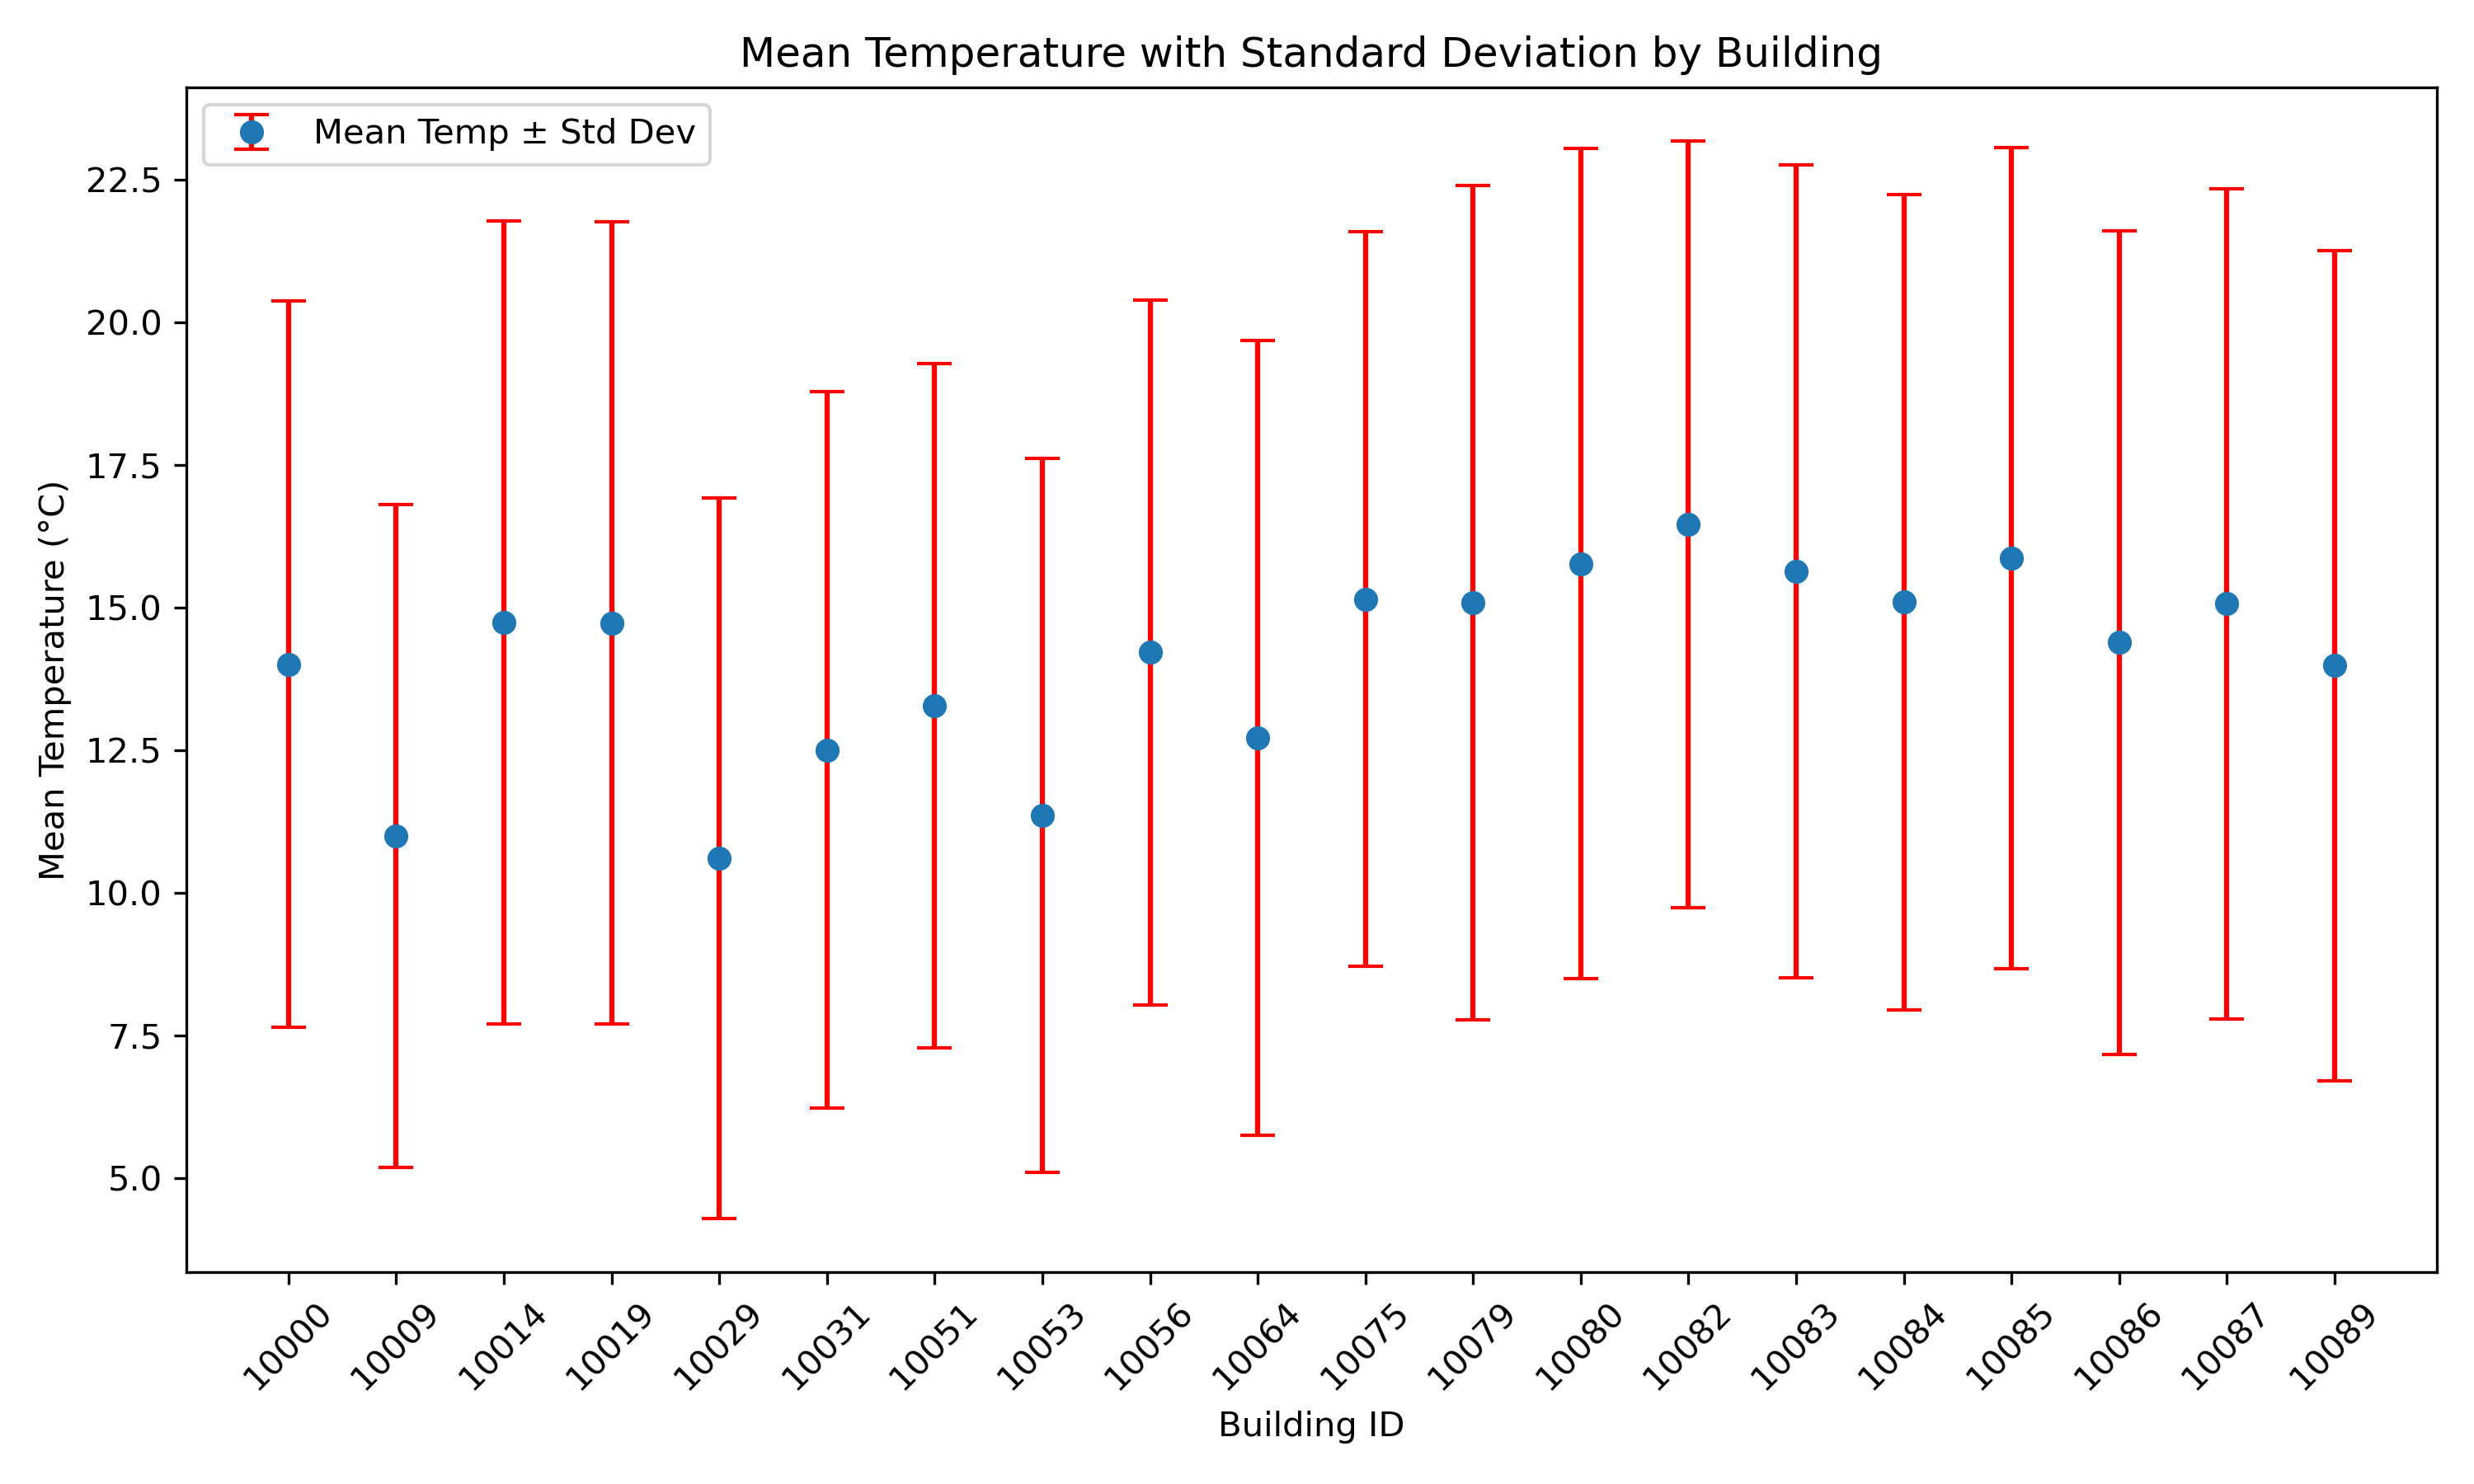
\includegraphics[width=1\textwidth]{Plots/mean_temp_with_std_dev.png}
                \caption{Temperature distribution across the 20 floor plans.}
                \label{fig:temperature_distribution}
        \end{figure}

        \item Areas with temperatures above 18ºC are considered safe from mold risk.
        \item Areas with temperatures below 15ºC are deemed too cold for human comfort, as seen on Figure~\ref{fig:temperature_distribution_precentage}.
        \begin{figure}[h!]
                \centering
                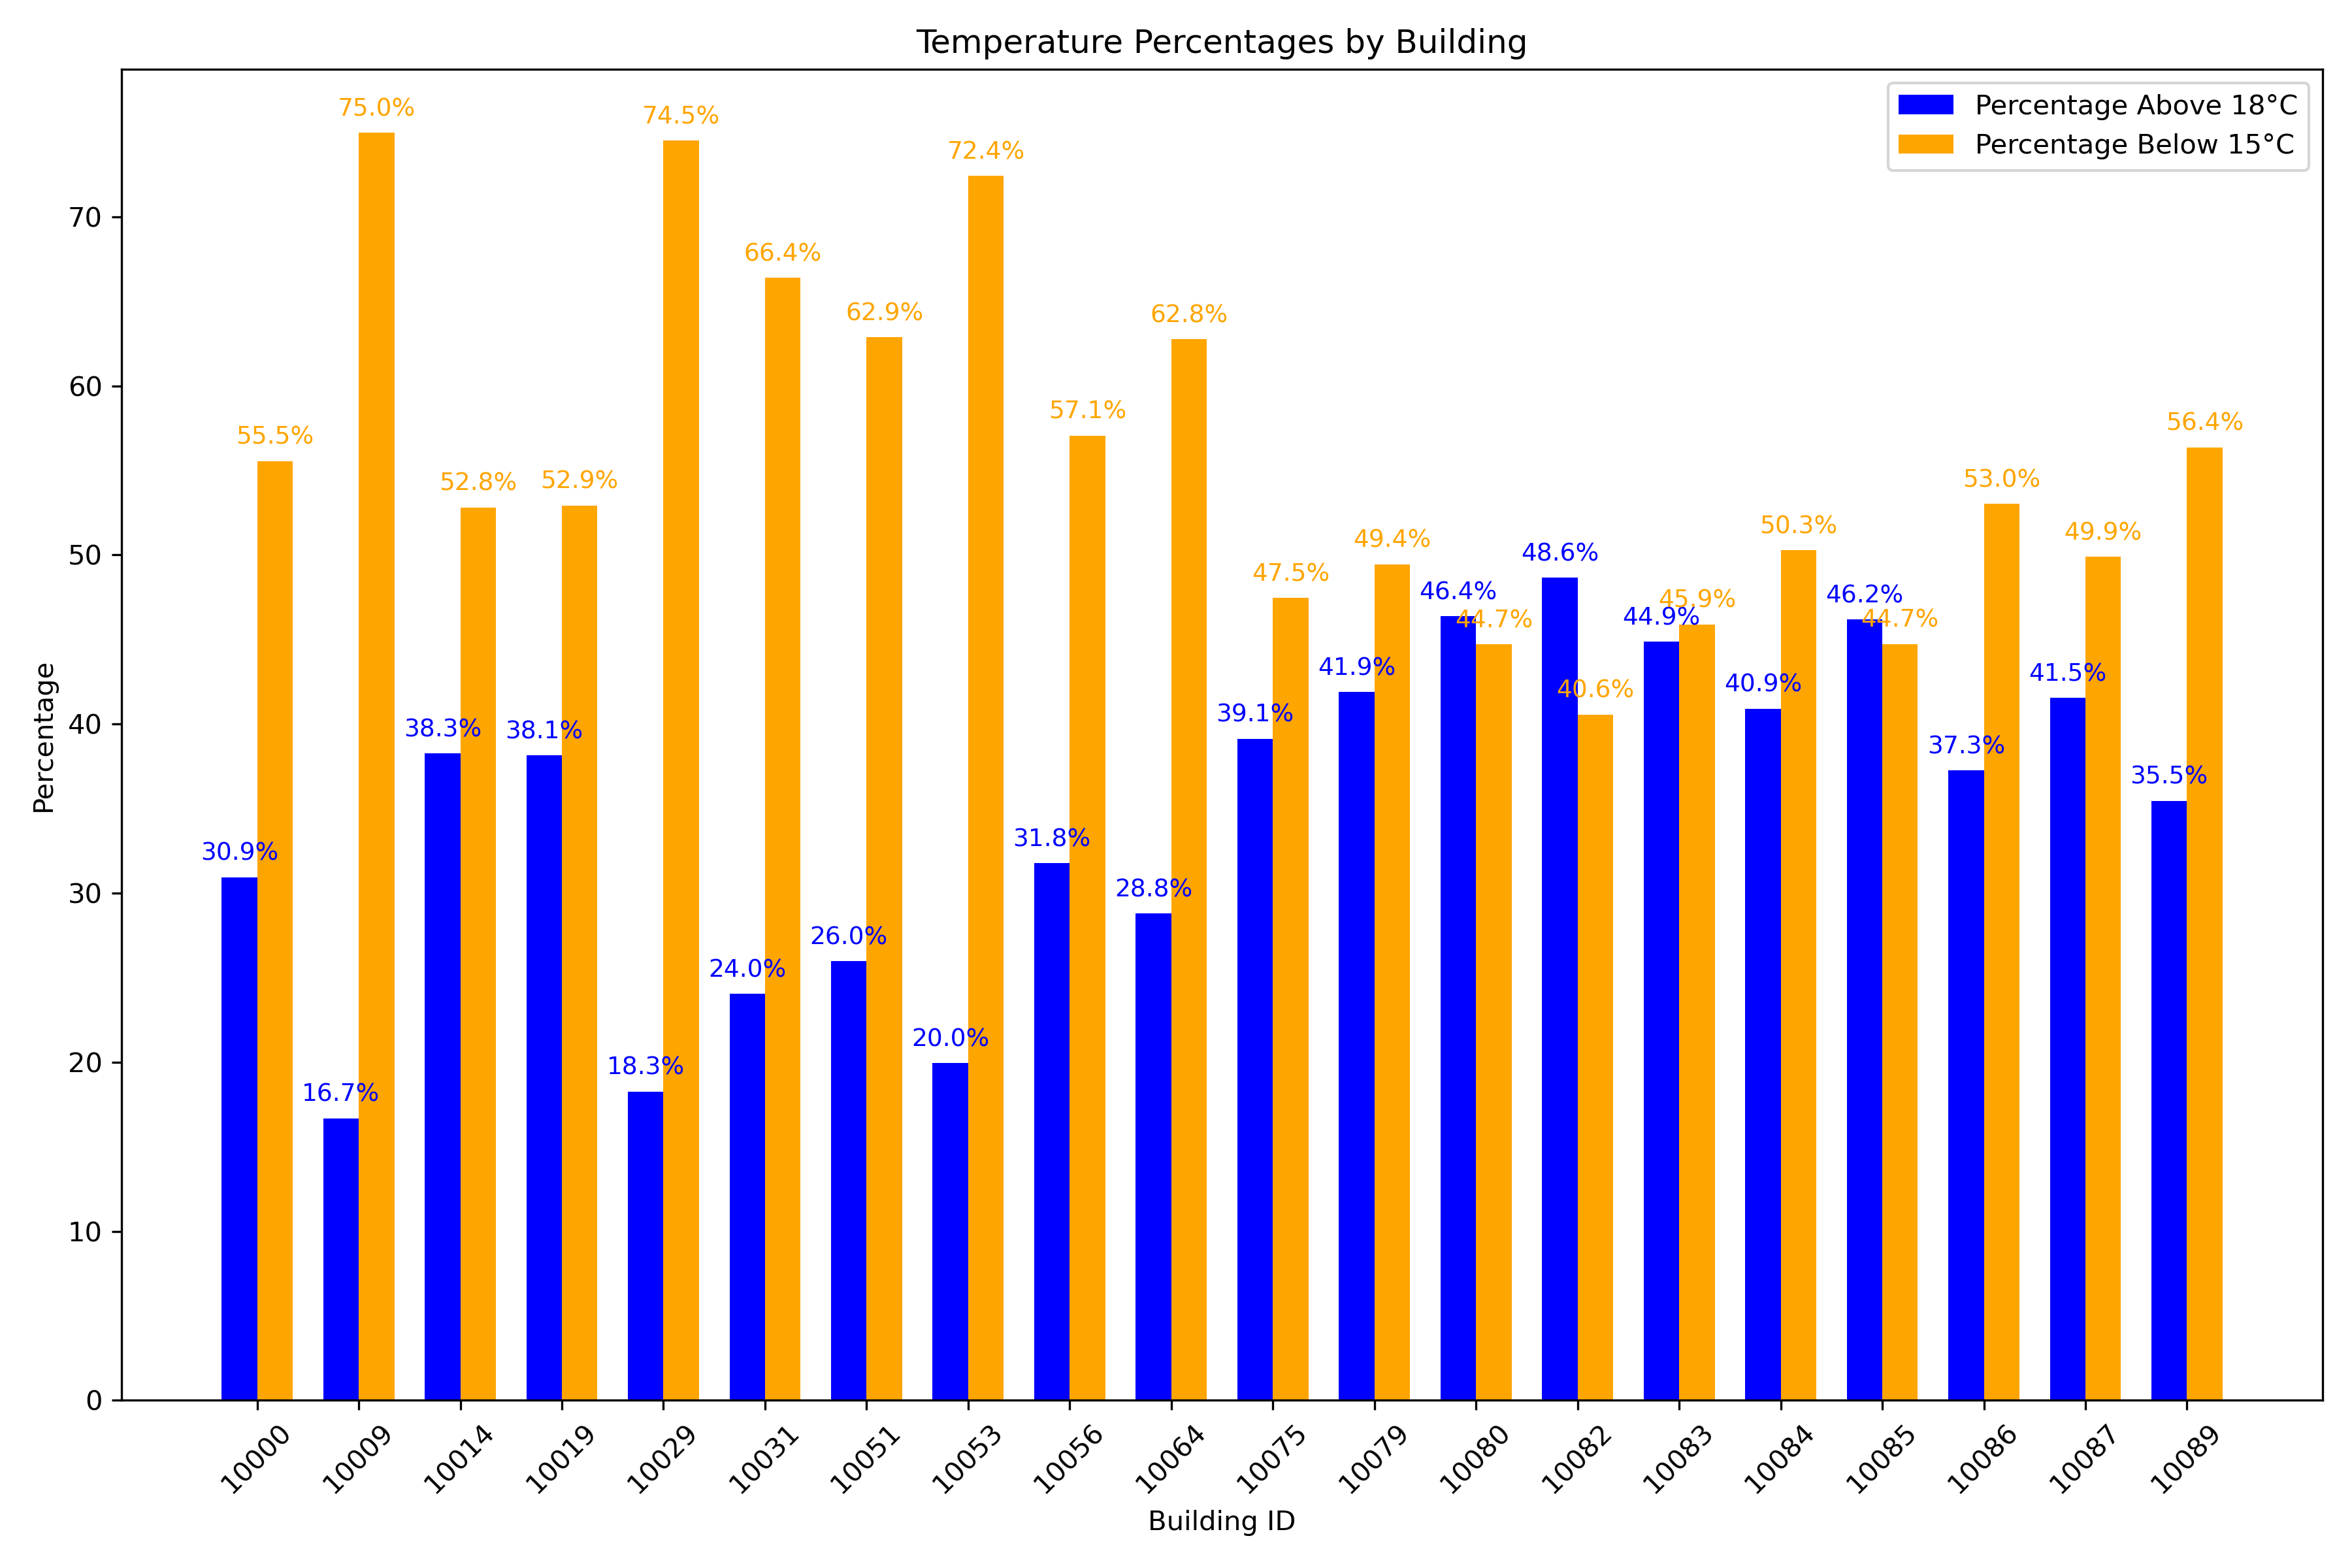
\includegraphics[width=1\textwidth]{Plots/temperature_percentages_by_building.png}
                \caption{Percentage of areas with different temperatures across the 20 floor plans.}
                \label{fig:temperature_distribution_precentage}
        \end{figure}

\end{itemize}


\subsection{Task 4}


\end{document}
